\section{Formalization}
In this section we first present our specification language and then
introduce the opeational semantics of our tool. The operational semantics of our tool is presented in two different sets. First set of rules, presents the core of our algorithm and we use it to present the proofs of correctness and optimality. 

\subsection{Specification Language}
Following is the formal syntax of contract language in our system:
\begin{figure}[t]
\begin{subfigure}{0.41\textwidth}
\centering
  \begin{fmathpar}
  \begin{array}{lclcl}
		\rel & \in & \texttt{rel.seed} & \coloneqq & \visZ \ALT
		\soZ \ALT \rel \cup \rel \\
               \Rel & \in & \texttt{relation} & \coloneqq &  \rel
	       \ALT \Rel;\rel  \ALT \nullR  \\
	     \pi & \in & \texttt{prop} & \coloneqq & \forall a.
      ~a \xrightarrow{R} \hat{\eff} ~\Rightarrow~ a \xrightarrow{\visZ}
      \hat{\eff}\\
		\psi & \in & \texttt{spec} & \coloneqq & \pi \ALT \pi \conj \pi
  \end{array}
  \end{fmathpar}
\subcaption{ syntax of contracts}
\label{fig:ctrt_syntax}
\end{subfigure}
\hfill \vline \hfill
\begin{subfigure}{0.49\textwidth}
\centering
\begin{scriptsize}
\begin{tabular}{|l | c |} 
\hline
 { \texttt Guarantee} & {\texttt Contract} \\ [0.5ex] 
\hline 
\textsc{Read My Writes} & $\forall a. a ~  ~\xrightarrow{\soZ}  ~ ~
\hat{\eta} \Rightarrow a \xrightarrow{\visZ} \hat{\eta} $ \\ 
\textsc{Monotonic Writes} & $\forall a. a \xrightarrow{\soZ;\visZ}
\hat{\eta} \Rightarrow a \xrightarrow{\visZ} \hat{\eta} $ \\ 
\textsc{Monotonic Reads} & $\forall a. a \xrightarrow{\visZ;\soZ}
\hat{\eta} \Rightarrow a \xrightarrow{\visZ} \hat{\eta} $ \\ 
\textsc{Transitive Visibility} & $\forall a. a \xrightarrow{\visZ;\visZ}
\hat{\eta} \Rightarrow a \xrightarrow{\visZ} \hat{\eta} $ \\ 

\hline
\end{tabular}
\end{scriptsize}
\subcaption{examples 
%({\bf R}ead {\bf M}y {\bf W}rites, {\bf M}onotonic
%{\bf W}rites and
%{\bf M}onotonic {\bf R}eads)
}
\label{fig:ctrt_example}
\end{subfigure}
\caption{\tool Specification Language}
\end{figure}

\\ The language is general enough to cover all  the known consistency
levels in the context:
\begin{figure}[h]
  \begin{smathpar}
  \begin{array}{ll}
		\texttt{ Read My Write (RMW): }  & \forall(a,b). a \xrightarrow{so} b ~\Rightarrow~ a \xrightarrow{\visZ} b\\
		\texttt{ Monotonic Reads (MR): }  & \forall(a,b). a \xrightarrow{so;vis} b ~\Rightarrow~ a \xrightarrow{\visZ} b\\
		\texttt{ Monotonic Writes (MW): }  & \forall(a,b). a \xrightarrow{vis;so} b ~\Rightarrow~ a \xrightarrow{\visZ} b\\
		\texttt{ Writes Follow Reads (WFR): }  & \forall(a,b). [a \xrightarrow{vis;vis} b ~\Rightarrow~ a \xrightarrow{\visZ} b] \wedge  
		[a \xrightarrow{vis;so;vis} b ~\Rightarrow~ a \xrightarrow{\visZ} b]\\


  \end{array}
  \end{smathpar}
\caption{Well-known consistency requirements, written in our specification language}
\label{fig:ctrt}
\end{figure}

\\ Contracts written in our language, can be visualized by simple graphs. For example, \texttt{(MR)} contract from the above figure can be represented as:
\begin{figure}[h]
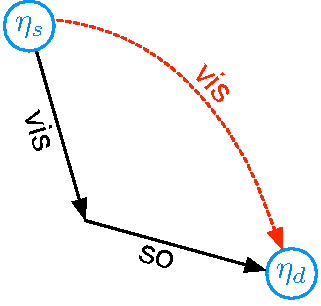
\includegraphics[scale=0.6]{../Figures/MR.pdf}
\caption{A simple way of showing contracts}
\label{fig:ctrt}
\end{figure}




\subsection{Core Algorithm Operational Semantics}
Here we explain the the core operational semantics of our algorithm, which for simplicity reasons, 
is parametrized over a single contract $\psi$:
\begin{smathpar}
\begin{array}{lcc}
\psi = \forall (a,b). a \xrightarrow{R} b  \Rightarrow a
\xrightarrow{vis} b, & \spc & R=r_1;r_2;...;r_k \\
\end{array}
\end{smathpar}
Before intorducing the semantics, let us define the inverse of a
given relation $R=r_1;r_2;...;r_k$.
The following definitions are parametrized over an execution $E$ and a set of \emph{available} effects V.
The idea is to define the inverse only if the \emph{necessary
information} about the sequence of relations, is available in V; this
way we can capture the reality of the distributed stores, where some
effects, carrying the required info about the relation being computed
might not be present at the moment.
\begin{smathpar}
\begin{array}{ccc}
   b \in (R;r_k)^{-1}_V (a) & \iff & \exists c.(c\in r_k^{-1} (a)) \wedge (b \in R^{-1}
   (c))  \wedge  (r_k^{-1}(a) \subseteq V)
\end{array}
\end{smathpar}
The above definition is based on the following definition of
the inverse of a clause :
\begin{smathpar}
r^{-1}(S) = 
\begin{cases}
\begin{array}{lll}
\bigcup^{}_{e\in S}. \{\eta|(\eta,e) \in E.r \} & if &r\in\{so,vis\} \\ 
r_1^{-1}(S)\cup r_2^{-1}(S) & if & r=r_1\cup r_2\\
G_{r}(S,\emptyset) & if &  r=r^* 
\end{array}
\end{cases}
\end{smathpar}
Where we define the helping function $G$ as follows: 
\begin{smathpar}
G_r(S,R) =
\begin{cases}
\begin{array} {lll}
G_r(r^{-1}(S,R\cup r^{-1}(S))) &if& r^{-1}(S) \neq \emptyset  \\
R  & &  otherwise
\end{array}
\end{cases}
\end{smathpar}
Given a set of effects, we also define its maximal closed subset
under the relation R as follows: 
\begin{smathpar}
\left \lfloor S \right \rfloor_V = S' \spc \mathtt{iff} \spc S'
\subseteq S \; \wedge \;
R_V^{-1}(S') \subseteq S' \; \wedge \; 
\not\exists
S''.((R_V^{-1}(S''))\subseteq S''\wedge |S''|>|S'|)
\end{smathpar}
\begin{figure}[t]
\raggedright
\textbf{Auxiliary Definitions}\\ \vspace{-2mm}
%
\begin{minipage}{0.5\textwidth}
\begin{fmathpar}
\begin{array}{lclcl}
  \multicolumn{5}{c}{
    {op} \in \mathtt{Operation\; Name} \spc \spc
    {v} \in \mathtt{Return\; Value} \spc \spc
    {s} \in \mathtt{Session\; Id} \spc\spc
  } 
  \\ 
  \eff & \in & \mathtt{Effect} & \coloneqq &  (s,op,v)\\
  F_{op} & \in & \mathtt{Op.\,Def.} & \coloneqq & \set{\eff} \mapsto v\\
  \EffSoup & \in & \mathtt{Eff\,Soup}	  & \coloneqq & \set{\eff} \\
  \visZ,\soZ &	\in & \mathtt{Relations} & \coloneqq & \set{(\eff,\eff)} \\
  {\E} 	& \in & \mathtt{Exec\;State}  & \coloneqq & \Exec \\
\end{array}
\end{fmathpar}
\end{minipage}
%

\vspace {3mm}

\textbf{Auxiliary Reduction} \; \\
\fcolorbox{black}{pgrey}{\scriptsize \(\auxred{S} {(\E,op_{<s,i>})} {} {(\E',\eff)}\)}\\
\begin{minipage}{0.9\textwidth}
\vspace{2mm}
\rulelabel{Oper}
\vspace{-2mm}
\begin{fmathpar}
\stretcharraybig
\begin{array}{l}
\RuleTwo
{
%\Theta(\rho \mapsto (v,cache)) \qquad
S \subseteq \EffSoup \qquad F_{op}(S) = v \qquad
\eta \not\in S \qquad
\eff = (s,op,v) \qquad  \\
%\id(\eta) = i \qquad
%\{\eff'\} = \EffSoup_{({\sf SessID}=s,\,{\sf SeqNo}=i-1)}\\
\EffSoup' = \EffSoup \cup \{\eff\}  \qquad
\visZ' = \visZ \cup S \times\{\eff\}\qquad
\soZ' = \soZ \cup \{(\eta',\eta) \,|\, \eta'\in \EffSoup_{({\sf
SessID}=s)}      \}\qquad
%\soZ' = (\soZ^{-1}(\eff') \cup \eff') \times\{\eff\} \cup \soZ
}
{
  \auxred {S} {((\EffSoup,\visZ,\soZ), op_{<s,i>}))}
  {} {((\EffSoup',\visZ',\soZ'),\eta)}
}
\end{array}
\end{fmathpar}
\end{minipage}
\vspace{4mm}\\
\textbf{Operational Semantics} \; \\
  \fcolorbox{black}{pgrey}{\scriptsize \((\E,op_{<s,i>}) \;\xrightarrow{V}\; (\E',\eff)\)}\\
\vspace{2mm}
\begin{minipage}{0.45\textwidth}
\rulelabel{UB Exec}
\vspace{-2mm}
\begin{fmathpar}
\stretcharraybig
\begin{array}{l}
\RuleTwo
{
  \visZ \subseteq r_k \spc
  V \subseteq E.A \spc  
  V'= \left \lfloor V \right \rfloor_V \spc
  \\ %   R^{-1}_{V}(\eta) \subseteq V' \\
  \auxred {V'} {(E, op_{<s,i>}))}
    {} {(E',\eta)} 
}
{
  (\E,op_{<s,i>}) \;\xrightarrow{V}\; (\E', \eff)
}
\end{array}
\end{fmathpar}
\end{minipage}
\hfill
\begin{minipage}{0.45\textwidth}
\rulelabel{LB Exec}
\vspace{-2mm}
\begin{fmathpar}
\stretcharraybig
\begin{array}{l}
\RuleTwo
{
     \visZ \not\subseteq r_k \spc
     V \subseteq E.A \spc  
     R^{-1}_{V}(\eta) \subseteq V \\
  \auxred {V} {(E, op_{<s,i>}))}
    {} {(E',\eta)} 
}
{
  (\E,op_{<s,i>}) \;\xrightarrow{V}\; (\E', \eff)
}
\end{array}
\end{fmathpar}
\end{minipage}
\\
\vspace{5mm}
\hrulefill\\
\caption{Core Operational semantics of a replicated data store.}
\label{fig:semantics}
\end{figure}


\newpage




\subsection {Shim Layer Operational Semantics}
In this section we introduce the complete behavior of our multi-consistenct shim layer as a new set of operational semantics. 
The rules are parametrized over a given map of operation names to
contracts, $\Psi :  op
\mapsto \psi $ and we assume each contract is of the form:
$\Psi(op)=\forall (a,b). a \xrightarrow{Q_{op}} \Rightarrow a \xrightarrow{vis} b.$ 
We use $Q_{op}[m]$ notation to refer to the m'th clause in the composition.
We define a pool to be a set of effects and a value that contains all
the effects that arrive to the replica. 
Our shim layer, also maintains a set of k caches (one cache for each
given contract). Each cache is maintained to be the largest
subset of pool that is closed under its
contract.  i.e. $\forall \eff \in \Cache(op). Q_{op}^{-1}(\eff)
\subseteq \Cache(op) $ 
\\We also maintain a level of availability for each effect
according to an operation and the current pool. If the availability of an effect for
$op$ is $x$, it means
that the effect satisfies the suffix of size $x$ of contract $\Psi(op)$.
An effect $\eta$ satisfies a suffix of size $x\geq 1$ of contaract
$\psi=\forall (a,b). a \xrightarrow{q_1;q_2;...;q_n} b$,
written as $ (\eta \models_{\Pool}^{x} \psi )$, if and only if
$(q_{n-(x-1)};...;q_{n} )^{-1}_{\Pool}(\{\eta\}) \subseteq \Pool$. The
initial availability value for all effects is 0, and increases when more
dependent effects arrive. 
\\
Following are the formal definitions: 
\\
\begin{minipage}{\columnwidth}
\begin{smathpar}
\stretcharraybig
\begin{array}{lclcl}
  \multicolumn{5}{c}{
    {\delta} \in \mathtt{Replicated\; Data\; Type} \spc\spc
    {v} \in \mathtt{Value}\spc\spc
    {op} \in \mathtt{Operation\; Name}
  }\\
  \multicolumn{5}{c}{
    {s} \in \mathtt{Session\; Id} \spc\spc
    {i} \in \mathtt{Effect\; Id} \spc\spc
    {\rho} \in \mathtt{Replica\; Id}
  }\\
  \eff & \in & \mathtt{Effect} & \coloneqq &  (s,i,op,v)\\
   {\Pool} & \in & \mathtt {Pool} & \coloneqq & (v,\set {\eff}) \\
   {\Cache} & \in & \mathtt {Cache} & \coloneqq & op \mapsto (v,\set{\eff})\\
   \Avail & \in & \mathtt {Avail} & \coloneqq & op \mapsto (\eff \mapsto
\{0,1,...,k-1\}) \\
  F_{op} & \in & \mathtt{Op.\,Def.} & \coloneqq & v \rightarrow \eta\\
  \EffSoup & \in & \mathtt{Eff\,Soup}	  & \coloneqq & \set{\eff} \\
  \visZ,\soZ &	\in & \mathtt{Relations} & \coloneqq & \set{(\eff,\eff)} \\
  {\E} 		& \in & \mathtt{Exec\;State}  & \coloneqq & \Exec \\
  \Theta  & \in & \mathtt{Store}      & \coloneqq & \rho \mapsto
  (\Pool, {\Cache}, \Avail) \\
  {\sigma} 	& \in & \mathtt{Session} 					 	& \coloneqq & \cdot \ALT op::\sigma \\
  \Sigma 		& \in & \mathtt{Session\;Soup}   	 	& \coloneqq &
        \langle s, i, \sigma \rangle \pll \Sigma \ALT \emptyset \\
\end{array}
\end{smathpar}
\end{minipage}
%
\begin{smathpar}
\begin{array}{c}
\ssn(s,\_,\_,\_) = s \spc\spc
\id(\_,j,\_,\_) = j \spc\spc
\oper(\_,\_,op,\_) = op \spc\spc
\rval(\_,\_,\_,n) = n\\
\end{array}
\end{smathpar}



\begin{figure*}[h]
\raggedright
%

\textbf{Auxiliary Definitions}\\
%
\begin{minipage}{\columnwidth}
\begin{smathpar}
\stretcharraybig
\begin{array}{lclcl}
  \multicolumn{5}{c}{
    {\delta} \in \mathtt{Replicated\; Data\; Type} \spc\spc
    {v} \in \mathtt{Value}\spc\spc
    {op} \in \mathtt{Operation\; Name}
  }\\
  \multicolumn{5}{c}{
    {s} \in \mathtt{Session\; Id} \spc\spc
    {i} \in \mathtt{Effect\; Id} \spc\spc
    {\rho} \in \mathtt{Replica\; Id}
  }\\
  \eff & \in & \mathtt{Effect} & \coloneqq &  (s,i,op,v)\\
   {\Pool} & \in & \mathtt {Pool} & \coloneqq & (v,\set {\eff}) \\
   {\Cache} & \in & \mathtt {Cache} & \coloneqq & (v,\set{\eff})\\
  F_{op} & \in & \mathtt{Op.\,Def.} & \coloneqq & v \rightarrow \eta\\
  \EffSoup & \in & \mathtt{Eff\,Soup}	  & \coloneqq & \set{\eff} \\
  \visZ,\soZ &	\in & \mathtt{Relations} & \coloneqq & \set{(\eff,\eff)} \\
  {\E} 		& \in & \mathtt{Exec\;State}  & \coloneqq & \Exec \\
  \Theta  & \in & \mathtt{Store}      & \coloneqq & \rho \mapsto (\Pool,\Cache) \\
  {\sigma} 	& \in & \mathtt{Session} 					 	& \coloneqq & \cdot \ALT op::\sigma \\
  \Sigma 		& \in & \mathtt{Session\;Soup}   	 	& \coloneqq &
        \langle s, i, \sigma \rangle \pll \Sigma \ALT \emptyset \\
\end{array}
\end{smathpar}
\end{minipage}
%

\begin{smathpar}
\begin{array}{c}
\ssn(s,\_,\_,\_) = s \spc\spc
\id(\_,j,\_,\_) = j \spc\spc
\oper(\_,\_,op,\_) = op \spc\spc
\rval(\_,\_,\_,n) = n\\
\end{array}
\end{smathpar}

\vspace{5mm}
\textbf{Auxiliary Reduction} \;
  \fbox{\(\auxred{v} {(\E,\langle s,i,op \rangle)} {} {(\E',\eff)}\)}\\

\begin{minipage}{\textwidth}
\rulelabel{Oper}
\begin{smathpar}
\stretcharraybig
\begin{array}{l}
\RuleTwo
{
%\Theta(\rho \mapsto (v,cache)) \qquad
F_{op}(v) = \eta \qquad
\ssn(\eta) = s \qquad 
\id(\eta) = i \qquad
%\{\eff'\} = \EffSoup_{({\sf SessID}=s,\,{\sf SeqNo}=i-1)}\\
\EffSoup' = \EffSoup \cup \{\eff\} \\
\visZ' = \visZ \cup S \times\{\eff\}\qquad
\soZ' = \soZ \cup \{(\eta',\eta) \,|\, \eta'\in \EffSoup \conj 
    \ssn(\eta')=s \conj \id(\eta')<i\}\qquad
%\soZ' = (\soZ^{-1}(\eff') \cup \eff') \times\{\eff\} \cup \soZ
}
{
  \auxred {v} {((\EffSoup,\visZ,\soZ), \langle s,i,op \rangle}
  {} {((\EffSoup',\visZ',\soZ'),\eta)}
}
\end{array}
\end{smathpar}
\end{minipage}


\vspace{5mm}
\textbf{Operational Semantics} \;
  \fbox{\((\E,\Theta,\Sigma) \;\xrightarrow{\eff}\; (\E',\Theta',\Sigma')\)}\\

\begin{minipage}{3in}
\rulelabel{Pool Refresh}
\begin{smathpar}
\stretcharraybig
\begin{array}{l}
\RuleTwo
{ 
  \eta \in \E.\EffSoup \spc
  \Theta(\rho) = (\Pool,\Cache) \spc
  \eta \not\in \Pool_e \\
  \Pool' = (apply \; \eta\; \Pool_v,\Pool_e \cup \{\eta\}) \spc \\
  \Theta' = \Theta[\rho \mapsto (\Pool',\Cache)]\\
}
{
  (\E,\Theta,\Sigma) \;\xrightarrow{\eff}\; (\E, \Theta', \Sigma)
}
\end{array}
\end{smathpar}
\end{minipage}

\vspace{5mm}
\begin{minipage}{2.8in}
\rulelabel{Cache Refresh}
\begin{smathpar}
\stretcharraybig
\begin{array}{l}
\RuleTwo
{
  \Theta(\rho) = (\Pool,\Cache) \spc \eta \in \Pool_e
  \\ \eta \not\in \Cache_e \spc
  \Cache'=(apply \; \eta \; \Cache_v ,\Cache_e \cup \{\eta\}) \\ \psi^{-1}
  (\eta) \subseteq \Cache_e
 \spc  \Theta' = \Theta[\rho \mapsto (\Pool,\Cache')]\\
}
{
  (\E,\Theta,\Sigma) \;\xrightarrow{\eff}\; (\E, \Theta', \Sigma)
}
\end{array}
\end{smathpar}
\end{minipage}
\hspace{12 mm}
\vspace{3mm}
\begin{minipage}{2.3in}
\rulelabel{Exec}
\begin{smathpar}
\stretcharraybig
\begin{array}{l}
\RuleTwo
{
  \auxred{\CacheFinder_{\psi}(\Theta(\rho))} {(\E,\langle s,i,op \rangle)} {} {(\E',\eta)}  \\
  \Theta(\rho) = (\Pool,\Cache) \spc \psi^{-1}(\eta) \subseteq \Pool_e  \spc
}
{
  (\E,\Theta,\langle s,i,op::\sigma \rangle \pll \Sigma) 
    \;\xrightarrow{\eff}\;
  (\E',\Theta,\langle s,i+1,\sigma \rangle \pll \Sigma) 
}
\end{array}
\end{smathpar}
\end{minipage}


\caption{Operational semantics of a replicated data store.}
\label{sem:oper}
\end{figure*}







